\newcommand\UPPERWIDTH{6em}
\newcommand\MIDWIDTH{3.5em}
\newcommand\WIDTH{2.5em}
\newcommand\SHADOW{30}

\resizebox{\textwidth}{!}{
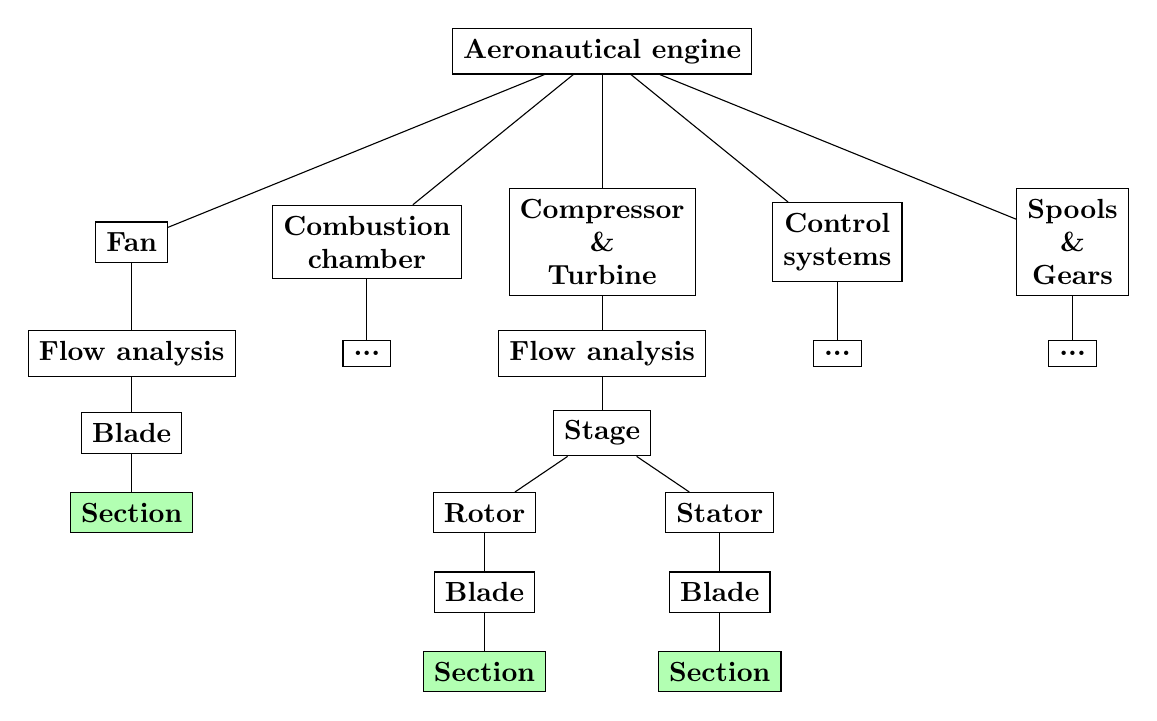
\begin{tikzpicture}[
    sibling distance=8.5em,
    every node/.style={
            shape=rectangle,
            draw,
            align=center,
            scale=1
        }
    ]

    \textbf{
    \node{Aeronautical engine}
        child[level distance=\UPPERWIDTH]{node{Fan}
            child[level distance=\MIDWIDTH]{node{Flow analysis}
                child[level distance=\WIDTH]{node{Blade}
                    child[level distance=\WIDTH]{node[fill=green!\SHADOW]{Section}}
            }}}
        child[level distance=\UPPERWIDTH]{node{Combustion\\chamber}
            child[level distance=\MIDWIDTH]{node{...}}}
        child[level distance=\UPPERWIDTH]{node{Compressor\\\&\\Turbine}
            child[level distance=\MIDWIDTH]{node{Flow analysis}
            child[level distance=\WIDTH]{node{Stage}
                child[level distance=\WIDTH]{node{Rotor}
                    child[level distance=\WIDTH]{node{Blade}
                        child[level distance=\WIDTH]{node[fill=green!\SHADOW]{Section}
                    }}}
                child[level distance=\WIDTH]{node{Stator}
                    child[level distance=\WIDTH]{node{Blade}
                        child[level distance=\WIDTH]{node[fill=green!\SHADOW]{Section}
                    }}}
            }}}
        child[level distance=\UPPERWIDTH]{node{Control\\systems}
            child[level distance=\MIDWIDTH]{node{...}}}
        child[level distance=\UPPERWIDTH]{node{Spools\\\&\\Gears}
            child[level distance=\MIDWIDTH]{node{...}}
    };
    }

\end{tikzpicture}
}